% !TEX program = xelatex
% =============================================================================
%  ICCIES 2027 submission (Springer CCIS / LNCS style)
%
%  Build with XeLaTeX only:
%      latexmk -xelatex main.tex     (or xelatex + bibtex + xelatex + xelatex)
%  latexmk picks the engine up from latexmkrc, so a bare `latexmk main.tex`
%  also works.
%
%  The Vietnamese examples carry tone-marked letters (lủ, nhục, sủa, mẹ) from
%  Unicode's Latin Extended Additional block, which T1/pdflatex cannot typeset:
%  it reports "Unicode character ... not set up for use with LaTeX" and drops
%  the letter, and the resulting Computer Modern setting needs 17 pages instead
%  of the 15 allowed.
% =============================================================================
\documentclass[runningheads]{llncs}

\usepackage{iftex}
\ifPDFTeX
  % Refuse to build: under pdfLaTeX the Vietnamese examples lose their tone
  % marks (T1 has no such glyphs) and the Computer Modern default needs 17 pages
  % instead of the 15 allowed.  \stop is required because Overleaf and editors
  % run TeX in nonstopmode, where \PackageError alone only prints the message and
  % then carries on producing a silently wrong PDF.
  \PackageError{iccies2027}{%
    Build this paper with XeLaTeX, not pdfLaTeX.\MessageBreak
    On Overleaf: Menu -> Compiler -> XeLaTeX.\MessageBreak
    Locally: latexmk -xelatex main.tex}{%
    Vietnamese tone marks do not exist in T1, so pdfLaTeX reports\MessageBreak
    "Unicode character ... not set up for use with LaTeX" for every example,\MessageBreak
    drops the letters, and needs 17 pages instead of the 15 allowed.}%
  \stop
\else
  \usepackage{fontspec}
  % TeX Gyre Termes is the TeX Live Times: metric-compatible with Times New
  % Roman and shipped with every TeX distribution, so the PDF is identical on
  % Overleaf and on Windows and needs no system font.  The font is loaded by
  % file name because name lookup of the texmf copy fails under MiKTeX.
  % Sans and mono stay at the class default (Latin Modern).
  \IfFontExistsTF{texgyretermes-regular.otf}
    {\setmainfont{texgyretermes}[
       Extension      = .otf,
       UprightFont    = *-regular,
       BoldFont       = *-bold,
       ItalicFont     = *-italic,
       BoldItalicFont = *-bolditalic]}
    {\setmainfont{Latin Modern Roman}}
\fi

\usepackage{graphicx}
\usepackage{booktabs}
\usepackage{array}
\usepackage{tabularx}
\usepackage{amsmath}
\usepackage{amssymb}
\usepackage{url}
\usepackage[hidelinks]{hyperref}

% The llncs class asks authors not to change the printing area or the caption
% spacing (llncsdoc, Sect. 2.1).  Only the float-placement policy and the
% separations around floats are relaxed here, so that five floats share the
% pages with the text inside the 15-page ICCIES limit; text geometry, heading
% and caption spacing keep the class defaults.
\renewcommand{\topfraction}{1.0}
\renewcommand{\bottomfraction}{1.0}
\renewcommand{\textfraction}{0.05}
\renewcommand{\floatpagefraction}{0.9}
\setcounter{totalnumber}{6}
\setlength{\textfloatsep}{5pt plus 2pt minus 2pt}
\setlength{\floatsep}{5pt plus 2pt minus 2pt}
\setlength{\intextsep}{5pt plus 2pt minus 2pt}
\setlength{\emergencystretch}{3em}

\newcommand{\model}[1]{\textsc{#1}}
\newcommand{\hate}{\textsc{hate}}
\newcommand{\off}{\textsc{offensive}}
\newcommand{\clean}{\textsc{clean}}

\begin{document}

\title{An Explainable Hybrid of Lexicon Rules and Multilingual
       Transformers for Vietnamese Hate Speech Detection}
\titlerunning{An Explainable Hybrid for Vietnamese Hate Speech Detection}

% ORCID iDs are optional in the class but expected by Springer for the
% corresponding author: replace the commented placeholders below with the real
% iDs (https://orcid.org) before submitting to CMT.
\author{
Kha Vy Pham\inst{1}% \orcidID{0000-0000-0000-0000}
 \and
Hong Nga Cao\inst{1}\textsuperscript{(*)}% \orcidID{0000-0000-0000-0000}
}

\authorrunning{K. V. Pham and H. N. Cao}

\institute{
FPT University, Can Tho, Vietnam\\
\email{phamkhavycm2004@gmail.com}\\
\email{caohongnga@gmail.com}\\
\textsuperscript{(*)}Corresponding author
}

\maketitle

\begin{abstract}
Fine-tuned multilingual transformers dominate Vietnamese hate speech detection,
yet they are opaque and brittle on the surface forms moderation sees: teencode,
dropped diacritics, inserted separators and abbreviated profanity.  We ask whether
a lexicon rule engine can be attached to such a transformer as an \emph{evidence
channel} rather than a competing classifier.  On the ViHSD test set (6{,}680
comments, 83\% \clean) we fuse a 668-term Vietnamese hate-speech lexicon, matched
through accent-less, leet, repeat-collapsed and separator-stripped views, with
four backbones that differ only in their optimisation recipe.  The headline effect
is small and not distinguishable from zero: the focused backbone improves from
0.6575 to 0.6602 macro-F1, a net of 8 comments (23 fixed, 15 broken),
with a paired-bootstrap $p=0.29$.  The value we report is not the delta but its
\emph{provenance}.  The rule channel fires on 15.75\% of test comments with
58.75\% precision, and all 23 corrections are rule-consistent: 16 \hate{}
recoveries where the rule fires in the corrected direction, and 7 \clean{}
de-flagging cases where it is correctly silent.  All 10 rule-driven regressions
push towards \hate{}, localising the failure mode to an aggressive channel rather
than to lexical coverage.  We further identify 132 missed corrections where the
rule already carries directional evidence fusion does not act on.  These
diagnostics, not the fourth decimal of macro-F1, are the contribution.
\keywords{Vietnamese hate speech \and ViHSD \and Explainable AI \and
          Hybrid fusion \and Lexicon rules \and Error analysis.}
\end{abstract}

\section{Introduction}
\label{sec:intro}

Vietnam has one of the fastest-growing social-media user bases in Southeast Asia and
the volume of Vietnamese text platforms must moderate keeps rising. The language
remains low-resource, and its social-media register is hard: writers abbreviate
profanity into \emph{teencode} (\texttt{dm}, \texttt{cc}, \texttt{vl}), drop
diacritics, stretch letters, insert separators inside words, and rely on irony or
quotation to be hostile without writing a dictionary slur.

The release of UIT-ViHSD \cite{luu2021vihsd}, roughly 33k comments labelled
\clean{}, \off{} or \hate{}, made supervised transformer fine-tuning the default
approach. Monolingual encoders such as PhoBERT \cite{nguyen2020phobert} and
ViSoBERT \cite{nguyen2023visobert}, multilingual DeBERTa-v3 variants
\cite{he2021deberta,he2023debertav3,liu2024mdeberta} and task-specific systems
\cite{nguyen2024vihatet5} all perform well, yet on ViHSD strong encoders plateau:
about 83\% of test comments are \clean{}, \hate{} and \off{} overlap in annotation,
and their boundary is often a matter of intensity rather than lexical content.

Two problems follow. The first is \emph{opacity}: a decision that removes a
comment needs a reason a moderator or appeals reviewer can inspect, yet post-hoc
attribution such as LIME \cite{ribeiro2016why} or SHAP \cite{lundberg2017shap}
approximates the model rather than describing the decision procedure. The second is
\emph{brittleness on surface form}: a transformer may never see \texttt{đm} written
as \texttt{d.m}, \texttt{đ*m} or \texttt{địt mẹ}, while a lexicon can be written to
match all of them explicitly.

We ask a narrow question: \emph{can a lexicon-based rule engine be attached to a
transformer as an evidence channel, so that every decision carries inspectable
lexical support, without degrading accuracy?} We do not claim that the hybrid is
more accurate: on the ViHSD test split the focused backbone improves by 0.0027
macro-F1, a paired-bootstrap $p$ of 0.29, a net of eight comments out of 6{,}680. We
claim something different and, for deployment, more useful: the small change is
\emph{attributable}. Every one of the 23 corrections and 15 regressions traces to a
specific mechanism, and the trace exposes a systematic failure that aggregate
metrics hide.

We fuse a 668-term Vietnamese hate-speech lexicon with four mDeBERTa-v3 backbones that
differ only in their optimisation recipe. The rule engine normalises the comment, builds
accent-less, leet, repeat-collapsed and separator-stripped views, scores each matched
span by severity, entry confidence, match type and context, and aggregates matches per
label; fusion mixes each channel and applies frozen per-channel thresholds.

The rule channel fires on 15.75\% of test comments at 58.75\% precision, supports all
23 corrections and drives all 10 rule-driven regressions; a further 132 \emph{missed
corrections} show the rule pointing right while the \clean{} channel blocks the fix.

The contributions are: (i) a frozen, reproducible hybrid protocol in which the rule
engine is an independent, inspectable channel rather than a competing classifier;
(ii) a per-decision provenance analysis assigning every changed decision to a
rule-driven or threshold-driven mechanism; (iii) a behavioural audit of the rule
channel with a multi-label cue taxonomy of the recovered \hate{} cases; (iv) the
identification of 132 missed corrections, which motivates evidence-gated rather than
score-averaged fusion; and (v) five case studies with matched spans and per-channel
scores.

\section{Related Work}
\label{sec:related}

\paragraph{Lexicon-based detection.}
Pre-transformer detectors used lexicons and hand-written surface features
\cite{waseem2016hateful}: Gitari et al.\ \cite{gitari2015lexicon} score a comment
from a curated profanity lexicon and apply rules over the matched phrases---inspectable,
but hand-curated, with recall bounded by the list. Wiegand et al.\
\cite{wiegand2018inducing} automate that induction step, the closest antecedent to how
our entries acquire severity and confidence. Schmidt and Wiegand's survey
\cite{schmidt2017survey} explains the move to learned models: the \hate{}/\off{}
boundary is combinatorial, not lexical. Davidson et al.\ \cite{davidson2017automated}
found the two classes share most of their surface vocabulary---the tension that makes
our channel over-fire on \off{}---and surveys \cite{fortuna2018survey} list the
recurring difficulties: imbalance, subjectivity, overlap, obfuscation, domain shift.
We take these as the object of analysis rather than as obstacles to a classifier.

\paragraph{Vietnamese resources and models.}
ViHSD \cite{luu2021vihsd} is the reference three-way benchmark, ViCTSD
\cite{nguyen2021victsd} provides related data, and ViCM \cite{nguyen2026vicm} adds
code-mixed comments. PhoBERT \cite{nguyen2020phobert}
adapts RoBERTa to Vietnamese, ViSoBERT \cite{nguyen2023visobert} is pre-trained on
social media, and ViHateT5 \cite{nguyen2024vihatet5} casts the task as generation.
ViHOS \cite{hoang2023vihos} annotates the \emph{spans} that make a comment hateful,
the closest Vietnamese work to our notion of evidence; our spans come from a lexicon
matcher rather than human annotation, but the motivation is the same. SMTCE
\cite{nguyen2022smtce} standardises Vietnamese social-media evaluation, which is why we
report macro-F1 rather than accuracy alone.

\paragraph{Multilingual transformers.}
mBERT \cite{devlin2019bert} and XLM-R \cite{conneau2020xlmr} established multilingual
pre-training; DeBERTa \cite{he2021deberta} introduced disentangled attention and
DeBERTa-v3 \cite{he2023debertav3} adds ELECTRA-style pre-training, whose
\texttt{microsoft/\allowbreak mdeberta-v3-base} checkpoint \cite{liu2024mdeberta} we
fine-tune.

\paragraph{Explainability and hybrid systems.}
HateXplain \cite{mathew2021hatexplain} made human rationales and explanation quality
benchmark quantities. LIME \cite{ribeiro2016why} and SHAP
\cite{lundberg2017shap} are model-agnostic but do not guarantee that the highlighted
tokens are the ones the decision used. Our rule channel is part of the decision
function, so its matched spans are \emph{faithful by construction} for the lexical
component, while the neural component remains opaque. We differ in two ways: we fix
the accuracy question with a paired test and analyse provenance instead, and we
report the rule channel's own error profile and the direction of every rule-induced
change. To our knowledge, this per-decision provenance audit has not been reported
for Vietnamese hate speech.

\section{Data and Lexicon}
\label{sec:data}

\subsection{The ViHSD corpus}
\label{sec:vihsd}

We use UIT-ViHSD \cite{luu2021vihsd}, a corpus of Vietnamese social-media comments
annotated with three mutually exclusive labels: \clean{} (no offensive content),
\off{} (offensive language that does not target a protected group as hate speech)
and \hate{} (hateful or seriously derogatory content). The \off{}/\hate{}
distinction depends on target and intensity rather than on a particular word, so a
purely lexical rule engine is insufficient on its own.

After cleaning, the corpus contains 33{,}398 comments. We use the fixed split shipped
with the project, and every system---rule engine, backbone, fusion variant and
analysis script---reads the same files. Each run directory stores the SHA-256 digest
of the split it used and re-checks it before training, ruling out a silently
re-shuffled split. Training contains 24{,}046 comments (2{,}556 \hate{}, 1{,}605 \off{}, 19{,}885
\clean{}), validation 2{,}672 (270/212/2{,}190) and test 6{,}680 (688/444/5{,}548).

The test split is imbalanced: 83.05\% \clean{}, 10.30\% \hate{} and 6.65\% \off{}.
Accuracy is therefore a poor headline metric---a constant \clean{} predictor already
reaches 0.8305---so macro-F1 is primary, always reported with per-class F1. The
6{,}680 test rows contain 6{,}571 distinct texts, i.e.\ 109 duplicated rows. They
are kept because removing them would change the frozen test set; one appears twice
among the 15 regressions, which therefore cover 14 distinct texts.

\subsection{The hate-speech lexicon}
\label{sec:lexicon}

The rule engine is driven by a Vietnamese hate-speech lexicon of \textbf{668
entries}, mined and labelled from the \emph{training} portions of three corpora:
ViHSD; R-ViHSD, a cleaned release that adds TDTU YouTube and voz-forum comments to
ViHSD \cite{bontoriTdtu}; and the code-mixed ViCM corpus \cite{nguyen2026vicm}. The
three training splits yield 1{,}062 candidate terms, of which 257, 665 and 140 are first
attested in ViHSD, ViCM and R-ViHSD; labelling reduces them to the entries kept below.
No comment from any evaluation split contributes to the dictionary, and each entry
records which corpora supported it (414 of the 668 occur in all three).
Each entry stores the surface term and a canonical form, a lexical label (\hate{} or
\off{}) with a per-label severity, an entry confidence estimated from the training
data, a context-required flag, and a review status (\emph{verified} or
\emph{auto}); both statuses may match, but the flag is retained in the evidence
record.

The lexicon is deliberately not a list of slurs. Most entries---551 of 668
(82.5\%)---are multi-word constructions such as \emph{mả cha}, \emph{con mẹ} or
\emph{ngu hơn}, and 524 (78.4\%) are context-required, because Vietnamese insults
frequently work by comparison and implication rather than by a single taboo word.
Only 74 entries carry an \off{} lexical label against 594 for \hate{}, which is why the
rule engine is weak on \off{} and fusion keeps that channel mostly neural. Three
properties make the lexicon worth keeping: it is \emph{editable} (a new variant needs
no retraining), \emph{deterministic} (the same comment yields the same spans) and
\emph{inspectable} (each score decomposes into a term, a match type and a context
factor).

\paragraph{Ethics of examples.}
All quoted comments are public ViHSD test comments. Because they contain profanity
and slurs, we mask the offending characters with \texttt{*} in every table;
evaluation always runs on the unmasked text. No user identifiers are reproduced, and
names that occasionally appear inside comments are part of the public corpus text.

\section{Method}
\label{sec:method}

\begin{figure}[ht]
\centering
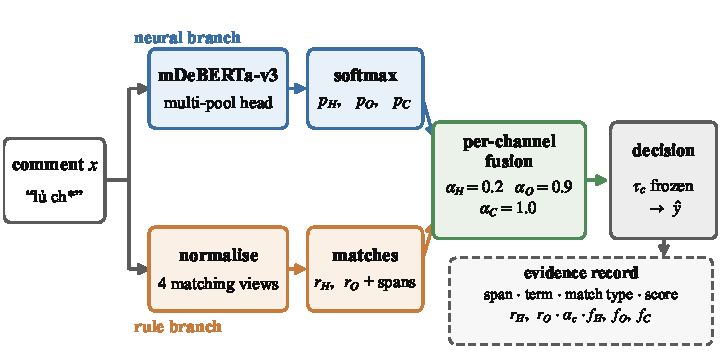
\includegraphics[width=\textwidth]{figures/architecture.pdf}
\caption{The hybrid. A comment enters two independent branches. The neural branch
produces class probabilities; the rule branch produces per-label lexical scores and
the spans that produced them. Fusion mixes each channel with its own weight
$\alpha_c$, and frozen per-channel thresholds turn the three scores into a label.
The evidence record is emitted with the decision and makes the lexical part of the
decision inspectable. Weights and thresholds shown are the values selected on
validation for the focused backbone.}
\label{fig:architecture}
\end{figure}

The hybrid has three parts: a rule engine that produces lexical scores and spans, a
transformer that produces class probabilities, and a fusion layer that combines them
channel by channel (Fig.~\ref{fig:architecture}). The branches share no parameters,
which allows the rule branch to be audited on its own.

\subsection{The lexical rule engine}
\label{sec:rule-engine}

\paragraph{Normalisation and views.}
The comment is Unicode-normalised to NFC, invisible characters are removed,
whitespace is collapsed, character runs are shortened to at most three, and the text
is lower-cased while keeping Vietnamese diacritics. Normalisation returns an
\emph{offset map} to the raw comment, so a match on a cleaned view is always reported
as a span of the original text. Auxiliary views handle the writing tricks that matter:
accent-less, leet, repeat-collapsed, and a compact view with separators removed
(\texttt{n g u}). The matcher records, for every hit, the dictionary term, label, view,
raw span and a \emph{match type} (\emph{exact}, \emph{accentless\_alias}, \emph{leet},
\emph{repeat\_collapsed}, \emph{separator\_inserted}, \emph{obfuscated\_combined} or
\emph{fuzzy}).

\paragraph{Scoring.}
Every match $i$ receives
\begin{equation}
s_i \;=\; \sigma_{\ell(i)} \cdot c_i \cdot m_i \cdot \kappa_i ,
\label{eq:match}
\end{equation}
where $\sigma_{\ell(i)}$ is the severity of the matched label ($0.95$ for
\hate{}, $0.60$ for \off{} after tuning), $c_i$ the entry confidence from the
training split, $m_i$ the match-type factor and $\kappa_i$ a context factor for
quotation, negation and context-required terms. Matches of one label are
de-duplicated and aggregated with a saturating sum over at most $K=10$ matches:
\begin{equation}
r_\ell \;=\; 1-\prod_{i\in T_\ell}\left(1-s_i\right).
\label{eq:aggregate}
\end{equation}
For fusion they become a three-channel pseudo-probability
\begin{equation}
\tilde{\mathbf r} \;=\; \frac{1}{1+\min(r_H,r_O)}
\begin{bmatrix} r_H \\ r_O \\ 1-\max(r_H,r_O) \end{bmatrix},
\label{eq:pseudo}
\end{equation}
which preserves the ordering of the two toxic channels while placing \clean{} on
the same scale. When the rule is silent, $\tilde{\mathbf r}=(0,0,1)$: no evidence
is treated as maximal cleanliness evidence, the assumption that
Sect.~\ref{sec:analysis} tests.

\paragraph{Tuning.}
Scoring weights are tuned on validation by greedy coordinate descent, with
thresholds re-optimised for every candidate; test is never loaded. The search made
the engine more aggressive: severity \hate{} rose to $0.95$, the accentless-alias
factor was driven to $0.0$, the repeat-collapsed factor to $0.4$, the
combined-obfuscation factor to $0.3$, and the negation and context-required
factors to $1.0$. Validation preferred \emph{more} matches over \emph{cautious} ones:
the engine is a narrow, high-threshold detector, not a comprehensive obfuscation
detector.

\subsection{The neural branch}
\label{sec:neural}

We fine-tune \texttt{microsoft/mdeberta-v3-base}
\cite{he2023debertav3,liu2024mdeberta}. The focused backbone
(\model{sensitiveai-vi-custom}) uses a multi-pool head: the final hidden states are
pooled with the \texttt{[CLS]} token, mean pooling and max pooling, the three views
are concatenated, projected to a 512-dimensional bottleneck with dropout $0.1$, and
mapped to three logits. Training uses cross-entropy, AdamW
\cite{loshchilov2019adamw}, a linear schedule with $10\%$ warm-up, learning rate
$3\times10^{-5}$, effective batch size 32, maximum length 256 and at most 30 epochs,
with early stopping on validation macro-F1; the best checkpoint is frozen before
test. Three further backbones use the same encoder with different recipes: a
standard-head baseline, a two-stage model with discriminative learning rates and
focal loss \cite{lin2017focal}, and a three-stage curriculum
\cite{bengio2009curriculum} with manual class weights.

\subsection{Fusion and decision}
\label{sec:fusion}

Let $p_c$ be the transformer probability for class $c$ and $\tilde r_c$ the
renormalised rule score. Per-channel fusion is
\begin{equation}
f_c \;=\; \alpha_c\,p_c \;+\; (1-\alpha_c)\,\tilde r_c,
\qquad c\in\{\hate{},\off{},\clean{}\}.
\label{eq:fusion}
\end{equation}
A single global $\alpha$ is the special case $\alpha_H=\alpha_O=\alpha_C$. A class
is \emph{accepted} when $f_c\ge\tau_c$; the accepted class with the highest $f_c$
wins, and if none is accepted the decision falls back to $\arg\max_c f_c$.

We compare four families: global $\alpha$ with argmax, global $\alpha$ with
thresholds, a multinomial logistic meta-classifier over the six AI and rule scores,
and per-channel $\alpha$ with thresholds. All tunable quantities are selected on
validation and frozen before the single test pass. The per-channel variant is
primary because the classes have different rule behaviour: the rule channel is
precise on \hate{}, weak on \off{} and uninformative on \clean{}, so one $\alpha$
forces a bad compromise. Validation discovers the asymmetry: $\alpha_H=0.2$,
$\alpha_O=0.9$, $\alpha_C=1.0$, with
$\tau_H=0.14$, $\tau_O=0.66$, $\tau_C=0.60$. The \hate{} channel is 80\% lexical,
\off{} 90\% neural and \clean{} purely neural; the interaction between
$\alpha_H$ and $\tau_H$ drives Sect.~\ref{sec:analysis}.

\subsection{Evidence record and protocol}
\label{sec:evidence}

For every comment the system emits, with the label, an evidence record: matched
spans in the raw text, dictionary term and label of each span, matching view and
match type, per-match score, aggregated rule scores, per-channel weights and the
three fused scores. Given the record and the transformer probabilities, a reviewer
can recompute the decision exactly, which is what we mean by \emph{faithful by
construction} for the lexical channel; the neural contribution remains a black box,
and we do not claim otherwise. Every tunable quantity is frozen before the single test
pass, and the error analysis is descriptive and performed after it.

\section{Experimental Setup}
\label{sec:setup}

\subsection{Backbones and tuning}
\label{sec:backbones}

Table~\ref{tab:backbones} lists the four backbones. All use
\texttt{microsoft/mdeberta-v3-base}, the same tokenizer, split and evaluation code,
and differ only in the head and optimisation recipe. The focused model,
\model{sensitiveai-vi-custom}, is chosen because it gives the clearest positive net
effect (23 corrections against 15 regressions), not because it has the highest
standalone score: the strongest backbone, \model{sensitiveai-vi-dlr2stage}, reaches
0.6638 macro-F1 but is almost indifferent to fusion (3 corrections, 2 regressions),
which makes it a poor subject for a study of what fusion changes.

\begin{table}[ht]
\centering
\scriptsize
\setlength{\tabcolsep}{3.5pt}
\caption{The four backbones and the paired tests between AI-only and the hybrid.
All backbones share the encoder (\texttt{microsoft/mdeberta-v3-base}), tokenizer,
split and evaluation code and differ only in the optimisation recipe.
$\Delta=\text{AI}-\text{hybrid}$ in macro-F1, so a negative value favours the
hybrid; the 95\% interval is the paired-bootstrap percentile interval over
10{,}000 resamples. $b$ is the number of comments the AI gets right and the
hybrid gets wrong, $c$ the reverse; the last column is the exact McNemar $p$.}
\label{tab:backbones}
\begin{tabular}{lccccccc}
\toprule
Backbone (recipe) & AI & Hybrid & $\Delta$ & 95\% CI & $p_{\text{boot}}$ & $b/c$ & $p_{\text{McN.}}$ \\
\midrule
\model{sensitiveai-vi} (std.\ head)        & 0.6545 & 0.6494 & $+0.0051$ & $[-0.0020,\,0.0120]$ & 0.1592 & 61/30 & \textbf{0.0015} \\
\model{sensitiveai-vi-custom} (multi-pool) & 0.6575 & \textbf{0.6602} & $-0.0027$ & $[-0.0079,\,0.0027]$ & 0.2942 & 15/23 & 0.2559 \\
\model{sensitiveai-vi-dlr2stage} (2-stage) & \textbf{0.6638} & 0.6637 & $+0.0000$ & $[-0.0020,\,0.0024]$ & 0.9782 & 2/3 & 1.0000 \\
\model{sensitiveai-vi-curriculum} (3-stage) & 0.6590 & 0.6618 & $-0.0028$ & $[-0.0058,\,0.0004]$ & 0.0868 & 8/31 & \textbf{0.0003} \\
\bottomrule
\end{tabular}
\end{table}


Rule-engine weights are tuned by greedy coordinate descent over the scoring
parameters, with the three decision thresholds re-optimised on validation macro-F1
over a 101-point grid at every candidate; the search never touches the lexicon.
Fusion follows the same discipline: thresholds by coordinate descent over the same
grid for three rounds, per-channel weights by coordinate ascent from the AI-only
corner, and a multinomial logistic meta-classifier fitted on the six validation
features. All selected values are frozen before the test pass.

\subsection{Metrics and implementation}
\label{sec:metrics}

Macro-F1 is primary (Sect.~\ref{sec:vihsd}). We report accuracy and per-class
precision, recall and F1, and evaluate differences with two
paired tests: a paired bootstrap over comments (10{,}000 resamples) for the
macro-F1 difference \cite{efron1993bootstrap}, and an exact McNemar test on the
correctness contingency table \cite{mcnemar1947note}. The bootstrap asks whether
the aggregate metric moved; McNemar asks whether the pattern of individual
decisions changed.

The transformer uses PyTorch and Hugging Face Transformers
\cite{wolf2020transformers}; metrics follow the scikit-learn definitions and are
computed by one shared evaluator \cite{saito2015precision}. The rule engine is pure
Python, runs on CPU, and processes a comment in 0.20\,ms on average (median 0.15\,ms),
roughly 4{,}900 comments per second, so it can run on every comment rather than as
a sampled audit.

\subsection{Reproducibility}
\label{sec:repro}

The split is hashed and re-checked, the rule-engine evaluation directory is recorded in
the fusion metrics and re-read rather than recomputed, and the analysis script asserts
that the rule scores shipped with the fusion predictions match the frozen tuned output.
This is not cosmetic: an earlier version silently read the \emph{untuned} scores and
over-reported rule coverage by a factor of three.

\section{Results}
\label{sec:results}

\subsection{The hybrid does not improve accuracy}
\label{sec:no-accuracy-gain}

Table~\ref{tab:fusion-variants} reports every decision variant for the focused
backbone and Fig.~\ref{fig:results}(a) plots the same ordering. The AI alone reaches
0.6575 macro-F1 and 0.8762 accuracy; the primary
per-channel hybrid reaches 0.6602 and 0.8774, a gain of 0.0027 macro-F1 and eight
additional correct comments (5{,}861 versus 5{,}853). The gain is concentrated in
\hate{}: F1 rises from 0.5830 to 0.5906, driven by recall (0.5334 to 0.5494) at a
small cost in precision (0.6427 to 0.6385). \off{} and \clean{} do not pay for it
(0.4493 to 0.4494, 0.9403 to 0.9407): the change is an extension of \hate{} recall,
not a reallocation between classes.

The other variants locate the effect: per-channel weights add 0.0010 macro-F1 over
a single global weight (0.6583 to 0.6593) and thresholds a further 0.0009. The
logistic meta-classifier is \emph{worse} than the AI alone (0.6513): fitting six
features on 2{,}672 validation comments overfits the rule scores and shifts the
operating point towards \hate{} recall. Thresholds do make the rule engine usable
on its own---0.5258 macro-F1, identical standalone and inside the pipeline, against
0.4714 with argmax, which collapses on \off{}---but it stays far below the
transformer (0.8421 accuracy).

\begin{table}[ht]
\centering
\scriptsize
\setlength{\tabcolsep}{3pt}
\caption{Decision-level variants for the focused backbone
(\model{sensitiveai-vi-custom}) on the test split. Every variant reads the same
frozen scores; only the mixing and decision rule differ. The last row is the
paper's primary system. \emph{Per-class columns are F1}; the best macro-F1 is
in bold. The two rule-only rows
are scored inside the fusion pipeline on the renormalised rule scores; the
standalone rule engine, with its own thresholds, is reported in the text.}
\label{tab:fusion-variants}
\begin{tabular}{lccccc}
\toprule
System & Acc. & Macro-F1 & \hate & \off & \clean \\
\midrule
AI only (argmax)                      & 0.8762 & 0.6575 & 0.5830 & 0.4493 & 0.9403 \\
Rule only (argmax)                    & 0.8494 & 0.4714 & 0.4867 & 0.0000 & 0.9274 \\
Rule only (frozen thresholds)         & 0.8421 & 0.5258 & 0.4102 & 0.2389 & 0.9284 \\
\midrule
Fusion, global $\alpha$ (argmax)      & 0.8769 & 0.6583 & 0.5851 & 0.4490 & 0.9408 \\
Fusion, global $\alpha$ (thresholds)  & 0.8769 & 0.6583 & 0.5851 & 0.4490 & 0.9408 \\
Fusion, logistic meta-classifier      & 0.8626 & 0.6513 & 0.5818 & 0.4379 & 0.9341 \\
Fusion, per-channel $\alpha$ (argmax) & 0.8774 & 0.6593 & 0.5882 & 0.4488 & 0.9408 \\
Fusion, per-channel (thresholds)      & 0.8774 & \textbf{0.6602} & 0.5906 & 0.4494 & 0.9407 \\
\bottomrule
\end{tabular}
\end{table}


\begin{figure}[ht]
\centering
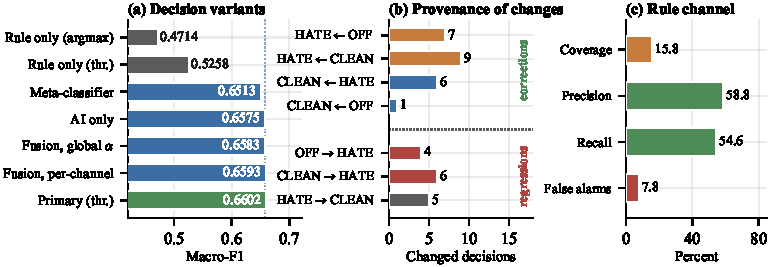
\includegraphics[width=\textwidth]{figures/results.pdf}
\caption{Quantitative summary for the focused backbone. (a)~Macro-F1 of every
decision variant; the dotted line is AI-only and the green bar is the primary
system. (b)~Provenance of the 38 changed decisions: the four correction types and
the three regression types. (c)~Behaviour of the rule
channel on the test split: coverage, precision when firing, recall on non-\clean{}
comments, and false alarms on \clean{}. Values are percentages; raw counts are in
the text and in panel~(b).}
\label{fig:results}
\end{figure}

\subsection{The difference is not distinguishable from zero}
\label{sec:significance-results}

Table~\ref{tab:backbones} makes the negative result explicit. For the focused
backbone the paired-bootstrap difference is $-0.0027$ with a 95\% interval of
$[-0.0079,+0.0027]$ and $p=0.29$; McNemar on the 38 changed decisions gives $b=15$,
$c=23$, $p=0.26$. Across the four backbones every bootstrap interval contains zero.
Where McNemar does reach significance the sign flips: the standard-head backbone
loses 61 comments to the hybrid and wins back 30 ($p=0.0015$), while the curriculum
backbone loses 8 and wins back 31 ($p=0.0003$). Fusion therefore helps one recipe and
hurts another by margins the aggregate macro-F1 cannot separate. We do not claim an
accuracy improvement: the hybrid is \emph{accuracy-neutral}, changing 38 decisions
without moving the aggregate metric beyond noise.

\subsection{The rule channel is narrow and precise-ish}
\label{sec:rule-channel-results}

The rule engine fires on 1{,}052 of 6{,}680 comments (15.75\%), not on the majority
of the test set. When it fires, 58.75\% of the comments are truly non-\clean{}, so
roughly two in five firings are false alarms; it recovers 54.59\% of non-\clean{}
comments and fires on 7.82\% of \clean{} comments (Fig.~\ref{fig:results}c). It is
useful as evidence, not as a decision: silent on 45\% of toxic comments and wrong
about a substantial share of those it flags. Coverage is low by construction---most
entries are multi-word, context-required phrases and validation zeroed the
accent-less alias weight---so the channel matches near-canonical forms rather than
respellings: narrow and inspectable rather than broad and opaque.

\section{Provenance and Error Analysis}
\label{sec:analysis}

The aggregate result is neutral; the question is what the 38 changes consist of.

\subsection{Corrections are rule-consistent}
\label{sec:corrections}

Of the 23 corrections, 16 are \hate{} recoveries (7 from \off{}, 9 from \clean{})
and 7 are \clean{} de-flagging cases (6 from \hate{}, 1 from \off{}). All 16 \hate{}
recoveries have a rule firing with a \hate{} score above the \off{} score, i.e.\ the
rule points in exactly the corrected direction. The rule \hate{} score has median
0.7652 (mean 0.7507, range 0.2351--0.9939), so the evidence is strong, not marginal,
for most of them.

All 7 \clean{} de-flagging cases have a silent rule ($r_H=r_O=0$, so
$\tilde{\mathbf r}=(0,0,1)$). With $\alpha_H=0.2$ the rule term disappears from the
\hate{} channel and $f_H=0.2\,p_H$, so a comment needs $p_H\ge0.70$ merely to reach
$\tau_H=0.14$; one flagged \hate{} at $p_H\approx0.5$ ends at $f_H\approx0.10$ and the
decision falls back to \clean{}, whose channel keeps the full neural weight
($\alpha_C=1$). The rule never touches the \clean{} channel, so silence acts only as a
multiplicative prior on \hate{}. We tested the alternative convention, where a silent
rule contributes nothing and the neural scores pass through unchanged: it changes 30
decisions (10 for it, 14 against) and raises macro-F1 from 0.6602 to 0.6614
(95\% CI $[-0.0015,+0.0042]$, $p=0.44$; McNemar 14--10, $p=0.54$). It is undecided,
so we keep the shipped convention for its net corrections ($+8$ against $+4$).

\subsection{Regressions are rule-driven and directional}
\label{sec:regressions}

The 15 regressions split into 10 rule-driven and 5 threshold-driven cases, and the
split aligns perfectly with direction (Fig.~\ref{fig:results}b). In all 10 rule-driven
cases (four
\off{}$\to$\hate{}, six \clean{}$\to$\hate{}) the rule fires in the \hate{}
direction, so fusion trusts lexical \hate{} evidence over the neural label and the
lexicon is wrong about intensity or target. The \off{} cases are the expected failure
of a phrase lexicon: profanity used as an intensifier rather than an attack. The
\clean{} cases are false positives on non-abusive text. One is a political comment
whose lexicon entry is a charged multi-word expression: the rule fires at $r_H=0.62$,
the transformer prefers \clean{} ($p_C=0.515$ against $p_H=0.473$), but the \clean{}
channel misses $\tau_C=0.60$ while the rule lifts $f_H$ to $0.588$, far above
$\tau_H=0.14$, so the decision goes to \hate{}. A lexicon entry's \emph{political}
sensitivity can therefore leak into moderation decisions
(Sect.~\ref{sec:discussion}).

The 5 threshold-driven regressions are the mirror image: the rule is silent, the
fused \hate{} score is $0.2\,p_H$, and when $p_H$ falls below roughly 0.7 the \hate{}
channel no longer wins; two miss by exactly 0.001 ($f_H=0.1390$ against
$\tau_H=0.14$). The symmetry is the point: one mechanism ($\alpha_H=0.2$,
$\tau_H=0.14$) produces 7 correct de-flagging decisions and 5 incorrect ones, and
cannot be removed without also removing the corrections. The decomposition is
exhaustive---26 of the 38 changes rule-driven, 12 threshold-driven---and that is what
makes the hybrid explainable: not a heat-map over the transformer but a statement of
which channel moved, in which direction, with which spans, and by how much.

\subsection{The corrections fusion does not make}
\label{sec:missed}

A channel with no signal and a channel whose signal fusion ignores look alike in an
aggregate; the second is the case here. Among the 827 AI errors, 148 non-\clean{}
comments have the rule firing in the correct direction and 151 \clean{} comments have
the rule correctly silent, so the rule agrees with the gold label on 299 errors.
Fusion acts on 23 of them (7.7\%). The remaining \textbf{132 missed corrections} are
non-\clean{} cases where the rule already points the right way and the hybrid is
still wrong. Separately, 144 of the 151 silent-\clean{} errors stay wrong because the
AI's \hate{} probability is high enough that even one fifth of it clears $\tau_H$.

The 132 are not missed because the lexical evidence is weak: their median rule
\hate{} score is 0.7609 (quartiles 0.67--0.85), indistinguishable from the 0.7652
median of the corrected cases. They are missed because the \clean{} channel keeps the
full AI weight ($\alpha_C=1.0$), so a confidently wrong \clean{} cannot be outvoted:
the median fused \clean{} score is 0.97 for missed cases versus 0.46 for corrected
ones.
Evidence-gated fusion (Sect.~\ref{sec:implications}) would abstain here; we did not tune
such a rule on test, which would invalidate the analysis.

\subsection{What the rule channel responds to}
\label{sec:cue-taxonomy}

We annotated the 16 \hate{} recoveries with a multi-label cue taxonomy: ten
contain teencode or abbreviated profanity (\texttt{đ*o}, \texttt{dm},
\texttt{cmnr}), five
standard-spelling profanity or an animal slur, and eight derogatory wording without
profanity (\emph{ngu}, \emph{thua}, \emph{nhục}); one has no surface cue. The
categories overlap, so the counts sum to more than 16. The channel is therefore not
merely a profanity detector: much of its value comes from derogatory wording a slur
list would miss, and teencode is its largest single category.

Which components do the work? Re-tuning and re-freezing the fusion once per switch
(Sect.~\ref{sec:fusion} protocol), only one switch matters: removing the per-entry
confidence costs 0.034 standalone macro-F1 (0.5258 to 0.4914), almost all of it on
\off{} (F1 0.2389 to 0.0600), and no other switch moves the standalone engine by more
than 0.008. Rescaling severity rewrites 1{,}046 of 6{,}680 rule scores yet changes no
hybrid decision ($p=1.0$): $\alpha$ and $\tau$ re-tune. Dropping the obfuscation
views trades recall for precision (firings
1{,}052 $\to$ 779, precision on fired comments 58.75\% $\to$ 69.58\%); fuzzy matching
never fires (0 matches), and case-folding cannot be ablated because all 6{,}680 test
comments are already lower-case. Inside the hybrid no switch leaves noise
($|\Delta|\le0.0012$): the channel helps as a channel, not through its weights.

\subsection{Case studies}
\label{sec:cases}

Table~\ref{tab:cases} shows five decisions covering these mechanisms. Case~1 is the
canonical rule rescue: two exact matches carry \hate{} from $p_H{=}0.19$ to
$f_H{=}0.81$, past the 0.78 \clean{} channel the AI is confident in. Case~2 is the one
correction in the five that the plain argmax would not make---\hate{} is 0.01 \emph{below}
\off{}, but \off{} falls short of its own $\tau_O{=}0.66$ while \hate{} clears
$\tau_H{=}0.14$, which is the 0.0009 that per-channel thresholds buy
(Table~\ref{tab:fusion-variants}). Case~3 is a de-flagging: a zero-weight accent-less alias
leaves the rule silent, the \hate{} channel collapses to $0.2\,p_H$, no channel clears
its threshold and the fallback returns \clean{}. Cases~4 and 5 are the two failure
modes of Sect.~\ref{sec:regressions}: an over-firing rule on profanity used as an
interjection, and a \hate{} channel that misses $\tau_H$ by exactly 0.001 and de-flags
a comment the AI got right.

\begin{table}[ht]
\centering
\scriptsize
\setlength{\tabcolsep}{3pt}
\renewcommand{\arraystretch}{1.0}
\caption{Case studies from the 38 changed decisions (\texttt{*} masks profanity).
$H/O/C$ are the fused channel scores, $\tau_c$ the frozen per-channel thresholds and
$r_H$ the aggregated \hate{} rule score; the figure after each span is its per-match
score. Rows 1--3 are corrections, 4--5 regressions.}
\label{tab:cases}
\begin{tabularx}{\textwidth}{@{}l>{\raggedright\arraybackslash}p{6.3cm}>{\raggedright\arraybackslash}X@{}}
\toprule
\# & Comment and rule evidence & Gold $\to$ AI $\to$ Hybrid \\
\midrule
1 & \emph{để avata bít ngay là ngu hơn chó} \newline $r_H{=}0.97$; ngu hơn 0.86, chó 0.79 (exact)
  & \hate{} $\to$ \clean{} $\to$ \hate{} \newline $H\,0.81 > C\,0.78$ \\
2 & \emph{\dots\ cũng đ*o thể yêu thương nổi} \newline $r_H{=}0.71$; cũng đ*o 0.71 (exact)
  & \hate{} $\to$ \off{} $\to$ \hate{} \newline $H\,0.49 < O\,0.50$ \\
3 & \emph{hóng bro tét đ*t thằng tùng} \newline $r_H{=}0$; accent-less alias, weight 0
  & \clean{} $\to$ \hate{} $\to$ \clean{} \newline $H\,0.10 < \tau_H{=}0.14$ \\
\midrule
4 & \emph{\dots\ nói không.. đợi cái loz} \newline $r_H{=}0.87$; cái loz 0.87 (exact)
  & \off{} $\to$ \off{} $\to$ \hate{} \newline $H\,0.70 > O\,0.68$ \\
5 & \emph{\dots abe tuổi lol mà so đc} \newline $r_H{=}0$; no scoring match
  & \hate{} $\to$ \hate{} $\to$ \clean{} \newline $H\,0.1390 < \tau_H{=}0.14$ \\
\bottomrule
\end{tabularx}
\end{table}


\section{Discussion}
\label{sec:discussion}

\subsection{What the hybrid is good for}
\label{sec:value}

The result is better read as a successful audit: 38 of 6{,}680 decisions change, each
described by a channel, a direction and a mechanism.

\emph{Triage and accountability.} A queue can sort comments by whether the decision was
rule-supported: a \hate{} decision with a matched span and $r_H=0.8$ is easier to review
than one with no lexical evidence, and the span, the entry and the arithmetic are what a
platform can defend in policy terms.

\emph{Editing and diagnosis.} Adding a slur variant is a configuration change, not a
retraining run, and an edit affects the \hate{} channel (weight 0.8) far more than the
others. The decomposition exists only because the channels are separate: a monolithic
classifier improving by 0.0027 macro-F1 would give no handle on whether the change was
lexical or neural.

\subsection{Why accuracy does not move}
\label{sec:why-neutral}

First, \emph{coverage is low}: the rule fires on 15.75\% of comments, so a perfect rule
channel could still only change decisions in that subset. Second, \emph{the majority
class dominates}: with 83\% \clean{}, only the 1{,}132 toxic comments can improve, and 38
changes is 3.4\% of that support---enough to matter operationally, too little to move a
macro-average beyond its confidence interval. Third, \emph{tuning is safety-oriented}:
protecting \clean{} and gating \hate{} on lexical support produces both the de-flagging
and the missed corrections. Neutrality is a \emph{choice}, not an absence of signal.

\subsection{The directional asymmetry is a policy question}
\label{sec:asymmetry}

In a binary ``remove / keep'' framing the asymmetry of
Sect.~\ref{sec:regressions} is a recall-oriented trade-off; in a three-class framing
it is not, because an \off{} comment mislabelled as \hate{} can trigger a stronger
sanction than the content warrants, and a political comment mislabelled as \hate{}
is a different kind of harm.

That false positive matters: the entry is a charged multi-word expression labelled
\hate{} from co-occurrence, so the lexicon is not a neutral artefact---it encodes
editorial judgments that enter at weight 0.8. Deployments should separate
\emph{profanity} from \emph{political} entries and weight them accordingly.

\subsection{Design implications}
\label{sec:implications}

Four changes follow. (i) \textbf{Evidence-gated fusion}: when the rule fires strongly
against a high-confidence \clean{} prediction, abstain or escalate. (ii) \textbf{Separate
thresholds per mechanism}: requiring $r_H\ge0.5$ before the \hate{} channel can override
would make the rule-driven and threshold-driven paths separately tunable. (iii)
\textbf{Per-class calibration} of the \clean{} channel, which currently blocks the missed
corrections. (iv) \textbf{Human-in-the-loop} for the 804 both-wrong comments, which no
fusion of these two channels can fix.

\subsection{Limitations}
\label{sec:limitations}

\paragraph{Single benchmark and language.} All results come from ViHSD and Vietnamese.
The lexicon and cue taxonomy are language-specific; the fusion protocol is not, but we
have not tested it elsewhere.

\paragraph{One seed per backbone.} Each backbone was trained once with seed 42, so
neural variance is not estimated and the 0.0027 difference is well inside what seed
variance could produce: the tests rule out a large effect, not a small one.

\paragraph{The rule engine is weaker than designed.} Validation set the accent-less
alias weight to zero and the negation factor to one, removing the main defence against
dropped diacritics and the discount for negated slurs visible in the
\off{}-as-intensifier regressions.

\paragraph{Explanations are not evaluated by humans.} The evidence record is faithful
for the lexical channel and decomposes the changed decisions, but we do not measure
whether reviewers find it useful, and the cue taxonomy is a post-hoc annotation.

\subsection{Ethics}
\label{sec:ethics}

The comments are public ViHSD test comments and are masked as described in
Sect.~\ref{sec:data}. The system is decision support, not automatic sanctioning: the
directional asymmetry and the political false positive show that automatic \hate{}
labels from this pipeline should be reviewed before they affect a user. The lexicon
should be treated as a governed artefact with a change log, because its entries shape
moderation outcomes.

\section{Conclusion}
\label{sec:conclusion}

We attached a 668-term Vietnamese hate-speech lexicon to four multilingual transformer
backbones as an evidence channel and evaluated it on the ViHSD test split. On the
focused backbone the hybrid improves macro-F1 from 0.6575 to 0.6602---a net of eight
comments, with paired-bootstrap $p=0.29$---so we do not present it as an accuracy
contribution.

The contribution is the provenance of the change. All 23 corrections are rule-supported
(16 \hate{} recoveries with median rule score 0.77, and 7 \clean{} de-flagging cases
where the rule is correctly silent), and all 10 rule-driven regressions push towards
\hate{}, localising the failure mode to an aggressive channel rather than to coverage.
A further 132 missed corrections show the rule already pointing right while a
full-weight \clean{} channel blocks the fix.

The broader lesson is methodological: a hybrid evaluated only by its aggregate metric
looks like a null result, whereas the same hybrid decomposed by channel and direction
yields an auditable decision procedure and a design agenda. Future work: validate
evidence-gated fusion, separate profanity from political entries, restore negation and
accent-less matching, and measure whether the evidence record helps reviewers.


% Credits go at the very end of the paper, just before the references
% (llncsdoc, Sect. 6).  The "Disclosure of Interests" paragraph is mandatory;
% an "Acknowledgments" paragraph (\ackname) may be added above it if the work
% was funded.
\begin{credits}
\subsubsection{\discintname}
The authors have no competing interests to declare that are relevant to the
content of this article.
\end{credits}

\bibliographystyle{splncs04}
\bibliography{references}

\end{document}
